\chapter{Variance Reduction for IMC Simulations of Astrophysical Events}

% Use the \AuthorBlock command to add the author and mentor names.
\AuthorBlock{Scott E. Campbell}{Mathew Cleveland, Kendra Long, and Ryan Wollaeger}

\begin{chapabstract}
	The Thermal Radiative Transfer (TRT) equations describe the coupling between thermal radiation and material, which is an important physical process in many problems of interest to the astrophysics community. The Implicit Monte Carlo (IMC) method, originally developed over 40 years ago~\cite{FC71}, is a standard solution methodology for the TRT equations. In this research, an improvement for IMC techniques for analyzing the interactions between a supernova and its circumstellar material is discussed, tested, and analyzed for a simplified geometry. This improvement uses a response function based variance reduction method to better estimate the observed time-dependent signal from a supernova system. The response function method improves the convergence, reliability, and accuracy of flux calcutions for different tally surfaces in IMC simulations. We were able to demonstrate said improvements by implementing this method in the open-source branson IMC code developed by Alex Long (\textit{along@lanl.gov}) using modern object-oriented languages.
\end{chapabstract}

\section{Introduction}
Electromagnetic (EM) transients are the main observational probe of supernovae, providing insight into the explosion energy, dynamics, and compositions of the exploding stars. These transients are formed by the complex interaction of photons with matter expanding at high velocity, and with a circumstellar medium (CSM) that existed before the supernova. Modeling supernovae with CSM interactions in multiple dimensions and extracting numerical transients is a challenging computational problem, requiring high spatial resolution in areas, relative to the overall distance between the star and CSM~\cite{MS10,MB13}. For the radiative transfer, in 1D deterministic~\cite{MB13} and Monte Carlo~\cite{KW09} have been applied to synthesize light curves and spectra.

However, to our knowledge, for 2D and 3D only simplified treatments of the radiation have been employed: parameterized radiative cooling~\cite{MS10,MK12}, the M1 moment closure approximation~\cite{VL16}, or no treatment (only hydrodynamics)~\cite{MP18}. Nevertheless, a spherical (or multidimensional) geometry can significantly impact the properties of the EM transient (spectra, light curves)~\cite{VL16,MP18}, and the effect of higher-order radiative transfer on the observables may be non-negligible.

Monte Carlo lends itself well to multiple dimensions since the sourcing of particles in space can be adjusted to mitigate transport in low-energy regions to efficiently resolve regions of phase space that are important to the observable quantities.

In a simulation of a multidimensional supernova interacting with a CSM, obtaining well-sampled multi-frequency, multi-observer-angle spectra may generally be prohibitively expensive with Monte Carlo, assuming escaping particles are directly tallied as part of the transient. For instance, assuming a modest $100^3$ cell 3D simulation, 10 observational views, and 100 observational wavelength bands, and further assuming 1\% of particles from each cell are tallied as escaping flux, the potential number of particles required to obtain 1 tally in each point in the observational phase space would be $\sim 100^3 \times 10 \times 100 \times 100 = 10^{11}$ particles.

Given the expense of simulating this number of particles, variance reduction that takes into account statistics at a tally surface (i.e. the ``telescope'') is worth exploring. Variance reduction methods are implemented to improve simulation efficiency while producing equivalent (unbiased) results. Such methods include implicit capture, splitting, Russian Roulette, and weight windows, which are described in more detail in Section~\ref{Sec: variance reduction}.

The remainder of this report outlines the background, motivation, and theory for the method, the algorithmic procedure, initial results, and an analysis of the cases and conditions where the method is useful.

\section{Background and Theory}
\subsection{Thermal Radiation Transport}
The absorption of a photon emitted from a material is described by the TRT equations:
\begin{equation} \label{Eq: TRT_1}
\frac{1}{c} \frac{\partial I}{\partial t}(\vec{r}, \vec{\Omega}, \nu, t) + \vec{\Omega} \frac{\partial I}{\partial \vec{r}}(\vec{r}, \vec{\Omega}, \nu, t) + \sigma_{a}(\vec{r}, \nu, T)I(\vec{r}, \vec{\Omega}, \nu, t) = 2 \pi \sigma_{a}(\vec{r}, \nu, T)B(\nu, T) + \frac{Q}{2}(\vec{r}, \nu, t),
\end{equation}
\begin{equation} \label{Eq: TRT_2}
c_{v}(\vec{r}, T) \frac{\partial T}{\partial t}(\vec{r},t) = \int_{0}^{\infty} \int_{-1}^{1} \sigma_{a}(\vec{r}, \nu^{\prime}, T)[I(\vec{r}, \vec{\Omega}^{\prime}, \nu^{\prime}, t) - 2 \pi B(\nu^{\prime}, T)] d \vec{\Omega}^{\prime} d \nu^{\prime}
\end{equation}
where $I$ is the specific intensity, $T$ is the material temperature (keV), $c$ is the speed of light, $B$ is the Planck function, $Q$ is the inhomogeneous source, $c_{v}$ is the material ssspecific heat, and $\sigma_{a}$ is the absorption opacity. Each of the terms in Eq.~\ref{Eq: TRT_1} corresponds to a loss or gain of photons from some phase space of the radiation field. The first term describes how the time behavior of the specific intensity depends on different gains and losses. The second is the streaming term, which describes how photons are lost by spatial streaming out of the phase space. The third describes the loss due to absorption into the material. On the right-hand side, the first is a gain term describing the radiation source from material temperature, and the second term then describes an arbitrary source of radiation. Equations \ref{Eq: TRT_1} and \ref{Eq: TRT_2} are non-linearly coupled with material temperature.

\subsection{Implicit Monte Carlo}
Monte Carlo methods are used to model time-dependent, nonlinear, radiative transfer problems in complex three-dimensional configurations. This stochastic numerical method uses random sampling to determine where and how a particle moves through a material. Some Monte Carlo methods minimize the effects of discretization errors through a continuous treatment of energy, space, and/or angle leaving the primary errors to be rooted in stochastic uncertainties. However, Monte Carlo methods typically come at the expense of long run times (with a standard convergence rate $\propto\frac{1}{\sqrt{N}}$, where $N$ is the number of histories simulated) and heavy use of machine resources.

The Implicit Monte Carlo (IMC) method is a specific variant of Monte Carlo originally developed by Fleck and Cummings in 1971 to solve the TRT equations~\cite{FC71}. IMC uses `effective scattering' to model particle absorption/re-emission in a material for its current time step. This is represented by the Fleck factor, $f$, described as follows:
\begin{equation}
f = \frac{1}{1 + \frac{4acT^{3}\sigma \Delta t}{c_{v}}}
\end{equation}
where $a$ is the radiation constant, $c$ is the speed of light, $T$ is the material temperature, $\sigma$ is the material opacity, $\Delta t$ is the time step, and $c_{v}$ is the material's specific heat.

The IMC method uses a semi-implicit time discretization of the emission term to linearize the system of equations. By linearizing the TRT equations, IMC takes on a maximum principle stability limit, that if violated, can result in unphysical behavior. Additionally, the time discretization is not fully implicit as implied, but rather semi-implicit as it is typically too expensive to converge otherwise.

In the \textit{branson} IMC code used for this research, the spatial domain is discretized into rectangular regions referred to as cells, each with a constant material temperature, radiation temperature, and density per timestep. Particles are tracked as they move through the cells and can be absorbed into the material, scattered, or stream out of the spatial domain. A particle is transported until it reaches the end of the time step or is fully absorbed by the material. Information about the system (e.g. fluence) is accumulated during the timestep and stored in a `tally'.

\subsection{Variance Reduction for IMC} \label{Sec: variance reduction}
Since the IMC method is stochastic, there will always be some statistical error in the result. Inherent issues with IMC methods include slow convergence and large computational requirements~\cite{AW16}. Furthermore, in cases where a material is optically thick and the distance from source to observation point (i.e. a tally surface) is large enough, the analog IMC method will fully absorb most particles into the material before they reach the tally, leaving the tally poorly sampled.

Due to these issues, variance reduction methods for IMC are necessary to provide equivalent answers while using fewer resources and converging faster. There are a large variety of variance reduction methods suited to different purposes. Common examples include implicit capture coupled with history termination, splitting and Russian Roulette, exponential transformation, forced collisions, source biasing, correlated sampling, optical reciprocity, and weight windows~\cite{JL16}.

Implicit capture, or absorption supression, is a classic variance reduction technique that adjusts a particle's weight at every collision event according to the following relationship:
\begin{equation}
w_{n,~i+1} = w_{n,~i}(1 - \frac{\sigma_{a}}{\sigma_{a} + \sigma_{s}})s
\end{equation}
where $\sigma_{a}$ and $\sigma_{s}$ are the absorption and scattering cross-sections, respectively. Implicit capture allows particle histories to exist longer in the problem, increasing the likelihood that a particle reaches a tally surface or other region of interest. 

Continuous absorption is similar to implicit capture, in that both extend particle histories by replacing analog absorption events with unbiased ``weight-change'' events.  Continuous absorption treats the particle energy-weight as a continuously-varying function of position. With the IMC Fleck factor, the expression for continuous absorption along a path segment is given bys
\begin{equation} \label{Eq: new_E}
E_{particle,~i+1} = E_{particle,~i}e^{-\sigma_{a} \cdot f \cdot d_{event}},
\end{equation}
where $d_{event}$ is the distance to the next position the particle travels to.  Continuous absorption is enabled by default in the \textit{branson} code.

Weight windows are another common variance reduction technique, in which each cell in the problem mesh is given a weight window center bounded by higher and lower values~\cite{JL16}. Once a particle enters a new cell, if a particle's weight is not within the weight window, one of two processes will occur. If the particle's wright is above the window, it will be split into additional particles. Particles whose weight is below the window will undergo a technique such as Russian Roulette~\cite{LM93} to remove the particle from the simulation.

All of the variance reduction methods listed above do not ensure that a tally surface will always be well sampled. In cases where particles have short mean free paths (i.e. traveling through a material with a high opacity), particles are still not guaranteed to pass through the tally surface. To ensure a tally is  well-sampled, ideally, all particles would contribute to the tally at least once before being fully absorbed into the material. To this end, a response function, in theory, will meet this requirement.

\subsection{Next Event Estimators}
Next event surface crossing estimators (NXTEVT) are an existing method for improving Monte Carlo tally statistics in radiation transport problems. To date, NXTEVT estimators have primarily been used in source-detector-type neutron transport problems. NXTEVT contributes to a tally surface the expected value of a particle that will cross through the tally surface. This method is an effective tool to minimize variance in situations where particles have limited histories, and large mean free paths in the problem material~\cite{WD11, LL99, LL05}. 

\begin{figure} [h!]
	\centering
	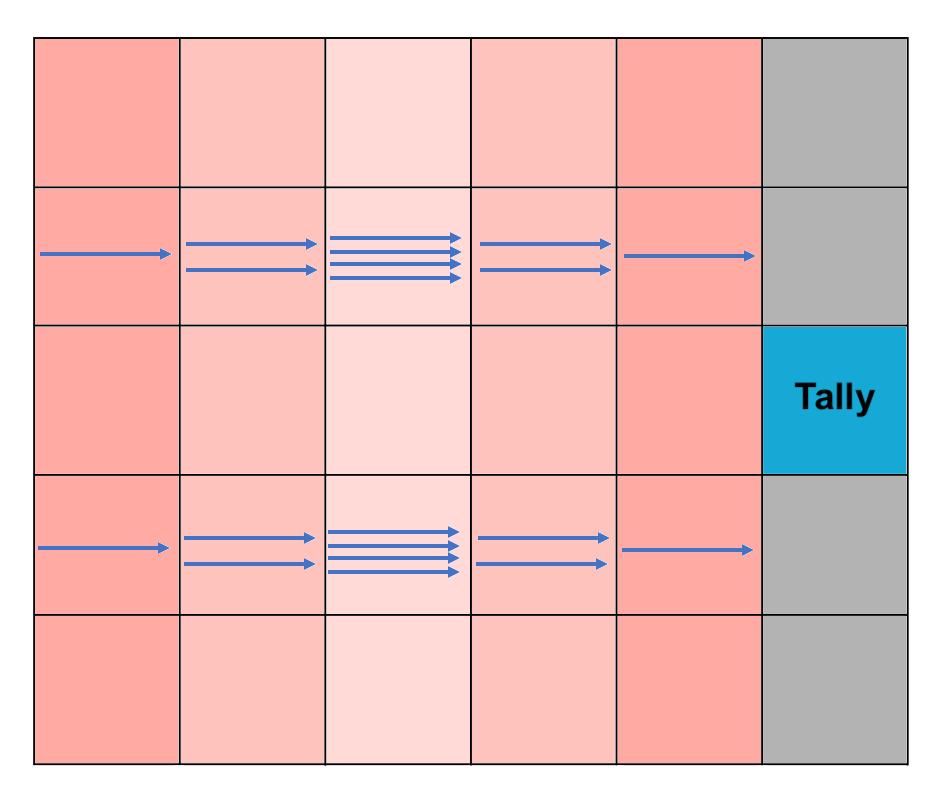
\includegraphics[height=3in]{VarReduction/plots/nxtevt_visual.png}
	\caption{A visual demonstrating why splitting is ineffective in optically thin regions: the split particles will all have generally the same direction and will stream with few collisions.}
	\label{fig:nxtevt_visual}
\end{figure}

NXTEVT estimators are implemented instead of splitting and Russian Roulette (e.g. weight windows) to get a well-sampled tally in small geometric regions. Figure \ref{fig:nxtevt_visual} demonstrates why splitting is ineffective in problems of low opacity. This method is preferred in cases where a limited number of particles reach an area of interest, i.e. tally. For example, this can result from optically thin regions where few collisions occur, mitigating scattering which would statistically direct more particles towards the tally region. In this case, particles will be transported further, and consequently, will deposit more energy and be rouletted before they reach they can reach the tally. Additionally, splitting and weight windows do not change a particle's direction, furthering the effects described earlier~\cite{BF12}.

This method points particles towards the region of interest to increase the sampling of important angles. The tally surface is 'scored' via the following equation: assuming that a particle is at a position $\vec{r}$, direction $\vec{\Omega}$, and weight $w_{0}$ intersecting a tally with a surface area $S_{tally}$ at a position $\vec{r^{\prime}}$ from the particle, the scored flux, $\phi(\mu)$, is given by
\begin{equation}
\phi(\mu) = w_{0} \frac{e^{-\int_{\vec{r}}^{\vec{r^{\prime}}} \Sigma_{t}(s)ds}}{S \cdot \mu}
\end{equation}
where $\mu$ is the angle between $\vec{\Omega}$ and the surface normal at $\vec{r^{\prime}}$, and $\Sigma_{t}$ is the total cross-section in the material. 

TRT has orders of magnitude more collisions and are typically solved on meshes rather than common editorial geometry. This makes the NXTEVT estimator very expensive. Because of these limitations, we chose to investigate a new method that adresses these issues. 

\subsection{Response Function Theory}
A response function can be an effective variance reduction method for tally surfaces because it contributes an adjusted energy value to the tally at every scatter event, rather than adding a contribution only once the particle passes through the tally surface. Because of this feature, the tally surface should be well-sampled using the response function compared to standard variance reduction methods. 

A response function estimates the probability that a particle `survives' to the tally surface following its current trajectory. The expected tally weight of the particle is proportional to the optical depth between the current particle position and the tally surface (in the direction of particle travel).

The response function is generated by tracing a number of particles through the problem domain starting uniformly on the tally surface, directed at a cosine-distribution angle. Since each cell may have a unique $\sigma_{a}$, every possible path from the source to the tally surface will result in a potentially unique contribution to the tally. The response function attempts to model this by averaging the absorption opacity based on the accumulation of all weighted $\sigma_{a}$ values from the previous cells into an effective opacity, $\sigma_{r}$. At every scattering event, the contribution of the particle to the tally is calculated by

\begin{equation}\label{Eq: tally_contr}
E_{contribution} = E_{particle}e^{-(\sigma_{r} + \frac{1}{c \Delta t})d_{tally}}
\end{equation}
where $E_{particle}$ is the current energy of the particle, $\Delta t$ is the current time step, and $d_{tally}$ is the distance of the particle to the tally surface along its path.

\subsection{Supernova and CSM Parameters} \label{sec:sncsmpars}
We attempt to model a snapshot of a supernova interacting with a circumstellar medium (CSM). The CSM has high enough mass to theoretically produce a superluminous supernova (e.g. SN 2006gy). The time for the snapshot is chosen to be after the supernova ejecta hits the CSM and produces a shock. This shock ionizes the CSM, which increases the opacity and consequently the optical depth. Moreover, the increase in density from the shock, coincident with the ionized region, also contributes to an increase in the optical depth of the CSM.

The approximate properties of each layer near the time of peak luminosity ($\sim70$ days) for model D2 of \cite{MB13} are as follows in Table~\ref{tab:supernova_params}.

\begin{table}[h!]
	\centering
	\begin{tabular}{lll}
		\toprule
		Supernova Ejecta & Ejecta-CSM Shock & CSM (pre-shock) \\ 
		\midrule
		$R_{\rm s, min} = 0$ cm & $R_{\rm s, min} = 10^{15.829}$ cm & $R_{\rm s, min} = 10^{15.831}$ cm \\ 
		$R_{\rm s, max} = 10^{15.829}$ cm & $R_{\rm s, max} = 10^{15.831}$ cm & $R_{\rm s, max} = 10^{16}$ cm \\ 
		$\rho_{\rm ej} = 10^{-14}$ g/cm$^3$ & $\rho_{\rm s} = 10^{-12}$ g/cm$^3$ & $\rho_{\rm CSM} = 10^{-14}$ g/cm$^3$ \\ 
		$T_{\rm ej} = 10^4$ K & $T_{\rm s} = 10^6$ K & $T_{\rm s} = 10^4$ K \\ 
		$c_v = 10^6$ erg/K/g & $c_v = 10^6$ erg/K/g & $c_v = 10^6$ erg/K/g \\ 
		$\kappa_{\rm ej} = 0.3$ cm$^2$/g & $\kappa_{\rm s} = 0.3$ cm$^2$/g & $\kappa_{\rm CSM} = 10^{-4}$ cm$^2$/g \\ 
		\bottomrule
	\end{tabular}
	\caption{}
	\label{tab:supernova_params}
\end{table}

For spherical symmetry, these values give masses of about 6, 8.5, and 14 for the interior ejecta, shocked ejecta-CSM, and CSM, respectively, which are on the order of the model values presented by M13. The optical depth through the internal ejecta is about 20, and is about 10 through the shocked ejecta-CSM layer. The preshock CSM is evidently hot enough to be ionized, hence it can contribute another 10 mean-free-paths of optical depth. The spatial width of the shock layer is only 0.46 \% of the radius of the shock, despite providing 1/3 of the total optical depth.

\subsection{Rescaling Parameters} \label{sec:rescaling}
We adjust dimensions and scale certain parameters to simplify setup of the supernova input. This can also be of use when attempting to test different types of supernovae conditions while preserving relevant physical properties or numerical resolution.

An adjustment of the overall domain size (radius),
\begin{equation}
\frac{R}{R_0} \approx 10^{-16} \;\;,
\end{equation}
where values subscripted with $0$ are unscaled, gives dimensions of O(1 cm). Relevant properties to preserve are the optical depth, light crossing time, and ratio of total time to the absorption-emission timescale. To preserve the light crossing time, we simply scale the total simulation time,
\begin{equation}
t = \frac{R}{R_0}t_0 \;\;,
\end{equation}
Similarly, assuming opacity is constant or piecewise-constant, the optical depth is preserved when
\begin{equation}
\kappa = \kappa_0\frac{R_0}{R} \;\;,
\end{equation}
where density has canceled from the left and right side. To preserve the ratio of the absorption-emission time scale to the total time, $t$,
\begin{equation}
t_{ae} = \frac{c_v}{4\kappa acT^4} = \frac{R}{R_0}t_{ae,0}
= \frac{R}{R_0}\frac{c_{v,0}}{4\kappa_0 acT^4} \;\;,
\end{equation}
which implies
\begin{equation}
c_v = c_{v,0} \;\;.
\end{equation}

Density and temperature have been left unchanged. The important aspect of this problem is the geometric structure and optical depth. To lower the spatial resolution requirements, the ejecta-CSM shock layer may be spread from 0.4\% to $\sim$10\% of the problem length while preserving optical depth. To do so, the density of the layer can be lowered to compensate for the increased size of the layer.

\section{Method and Technical Approach}
The implementation of the response function variance reduction method largely follows a standard Monte Carlo approach, with the addition of an inverse transport solve to generate the response function before running the forward transport problem. 

\subsection{Problem Initialization}	
At the start of the problem, several parameters are defined based on the properties of the materials in the problem domain. The absorption opacity, $\sigma_{a}$, is calculated using the Fleck factor:
\begin{equation}
\sigma_{a} = f \sigma.
\end{equation}The source emission, $S_{e}$ for each cell is defined as
\begin{equation}
S_{e} = c \cdot a \cdot \Delta t \cdot \sigma_{a}  \cdot T^{4},
\end{equation}
and total source emission, $S_{e,~total}$, is the sum of $S_{e}$ for each cell;
\begin{equation}
S_{e,~total} = \sum_{i = 1}^{n_{cell}} S_{e,~n}.
\end{equation}
The normalized weight, $w_{ideal}$, of each particle in the simulation is the quotient of $S_{e,~total}$ and $N_{particles}$. The number of particles to be emitted in each cell is then the quotient of $S_{e}$ and $w_{ideal}$. A check is run to ensure that each cell emits at least one particle. The time of emission for each particle is determined from a uniform distribution over the time step:
\begin{equation}
t_{0,~particle} = \xi \Delta t
\end{equation}
where $\xi \in [0,1]$ is a uniformly distributed random number. The temperature of each cell is calculated by
\begin{equation} \label{Eq: cell_T}
T_{cell} = \rho c_{v} \Delta t \Delta E
\end{equation}
where $\rho$ is the material density and $\Delta E$ is the difference between $S_{e}$ and the absorbed energy in each cell.

\subsection{Inverse Transport}
At the beginning of each time step, the response function is generated for the mesh. Our approach discretizes the function over the domain space, using each cell as a region to calculate the response opacity, $\sigma_{r}$. To calculate $\sigma_{r}$ for each cell, a set number of particles ($N_{response}$) are traced over the mesh to accumulate information. 

The first step is to initalize each particle. Each particle's starting position is initialized uniformly on the tally surface using the following equations:
\begin{equation} \label{Eq:pos_phi}
\phi = 2 \pi \xi ,
\end{equation}
\begin{equation}
\mu = 1 - 2 \zeta,
\end{equation}
\begin{equation} \label{Eq:pos_cost}
\theta = \arccos{\mu}
\end{equation}
where $\xi,~\zeta$ are uniformly-distributed random numbers, $\xi,~\zeta \in [0,1]$. The position vector, $\vec{r}$, is then given by
\begin{equation}
\vec{r} =
\begin{bmatrix}  
r_{0} \\
r_{1} \\
r_{2} \\
\end{bmatrix}
=
\begin{bmatrix}  
x_{tally} + R_{tally} \sqrt{1-\mu^{2}}  \cos{\phi}    \\
y_{tally} + R_{tally} \sqrt{1 - \mu^{2}} \sin{\phi}    \\
z_{tally} + R_{tally} \mu 										 \\
\end{bmatrix}
\end{equation}
where the tally is centered at $(x_{tally}, y_{tally}, z_{tally})$ with a radius of $R_{tally}$. 

Additionally, the direction of the particle is initialized towards the source via a cosine-distributed angle. First, the inward unit normal from the point to the source $\textbf{N}$ is given by:
\begin{equation}
\textbf{N} =
\begin{bmatrix}  
\hat{x} \\
\hat{y} \\
\hat{z} \\
\end{bmatrix}
= \frac{1}{n_{r}}
\begin{bmatrix}  
x_{tally} - r_{0}	\\
y_{tally} - r_{1}    \\
z_{tally} - r_{2}	 \\
\end{bmatrix}
\end{equation}
where $\frac{1}{n_{r}}$ is the unit vector fraction, $[(x_{tally}-r_{0})^{2} + (y_{tally}-r_{1})^{2} + (z_{tally}-r_{2})^{2}]^{\frac{1}{2}}$. Then an angle factor, $f_{angle}$, is calculated by:
\begin{equation}	
f_{angle} = \sqrt{|1 - \hat{z}^{2}|}   .
\end{equation} 
Lastly, the angle $\vec{\Omega}$ is:
\begin{equation}
\vec{\Omega} =
\begin{bmatrix}  
\hat{\Omega_{x}} \\
\hat{\Omega_{y}} \\
\hat{\Omega_{z}} \\
\end{bmatrix}
= \frac{1}{n_{\Omega}}
\begin{bmatrix}  
\hat{x} \cos{\theta} + \hat{z}\hat{x}\sin{\theta}\cos{\phi}f_{angle} - \hat{y}\sin{\theta}\sin{\phi}f_{angle}	    \\
\hat{y} \cos{\theta} + \hat{z}\hat{y}\sin{\theta}\cos{\phi}f_{angle} + \hat{x}\sin{\theta}\sin{\phi}f_{angle}	    \\
\hat{z}\cos{\theta} - f_{angle}\sin{\theta}\cos{\phi}	\\
\end{bmatrix}   .
\end{equation}
where $\phi$ is from Eq. \ref{Eq:pos_phi}, $\cos{\theta}$ is from Eq. \ref{Eq:pos_cost}, and $\frac{1}{n_{\Omega}}$ is the vector unit fraction, similar to above. 

\begin{figure} [h!]
	\centering
	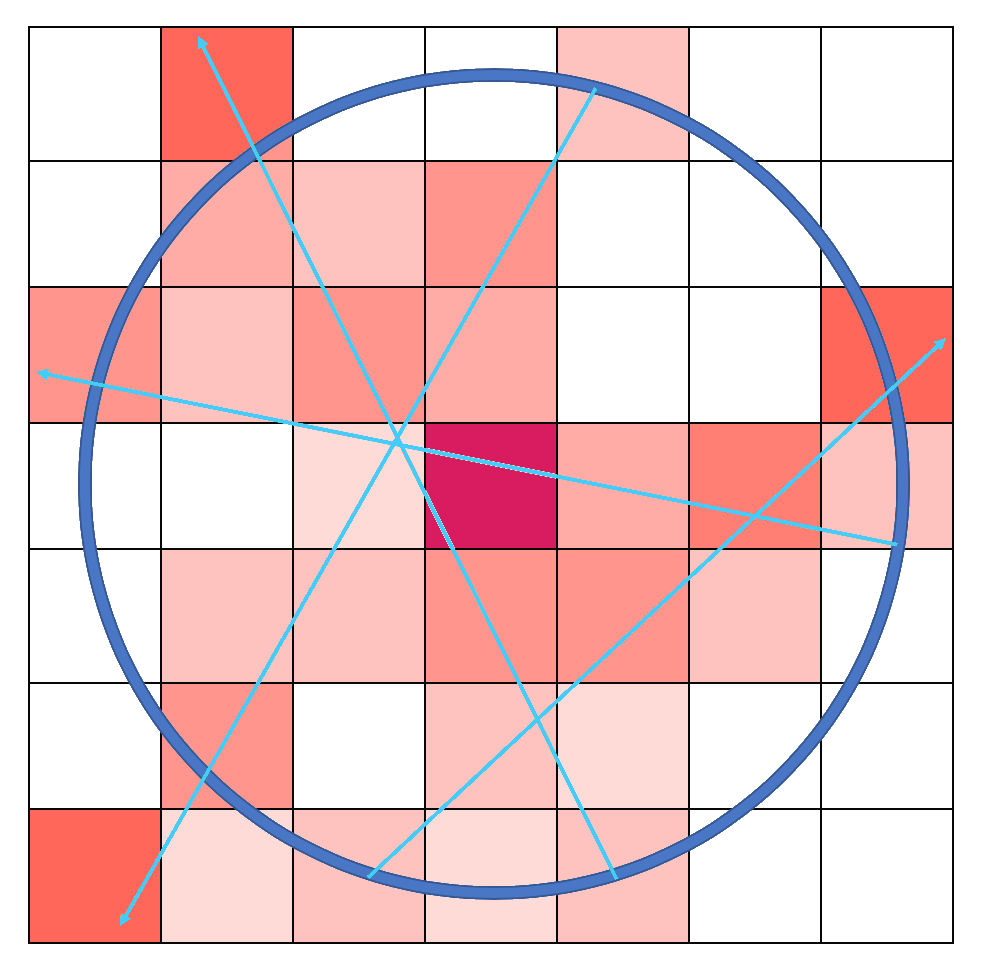
\includegraphics[height=3in]{VarReduction/plots/resp_funct_pt_src_vis.png}
	\caption{A simplified visualization of the response function method. Particles are traced from the surface of the tally (blue ring) ‘towards’ the source (purple square) until they exit the mesh. As the particle moves, an adjusted opacity, $\sigma_{r}$, is calculated based on how far the particle has traveled from its origin on the tally surface, as well as the $\sigma_{a,~cell}$ values of the cells that it has passed through. A darker shade of red corresponds to a higher $\sigma_{r}$ value – a less likely chance that a particle will ‘make it’ to the tally. These values are then used to calculate an effective contribution to the tally based on the cell the particle being transported is in.}
	\label{fig:resp_funct_visual}
\end{figure}

With the particle initialized, it is then traced through the mesh. Scattering and absorption events are not simulated. Instead, the following information is recorded as the particle passes a distance $d_{cell}$ through each cell:
\begin{enumerate}
	\item The total distance the particle has traveled through each cell, $d_{total,~particle} = \sum d_{cell}$.
	\item The sum of the distance the particle travels through each cell multiplied by the cells absorption opacity, $\sigma d_{total,~particle} = \sum d_{cell} \sigma_{a,~cell}$.
	\item The total distance, $d_{total,~cell} = \sum d_{n,~cell}$ for every particle $n$ that passes through each cell.
	\item The total distance multiplied by the absorption opacity, $\sigma d_{total,~cell} = \frac{\sigma d_{total,~particle}}{d_{total,~particle}} d_{cell}$ for every particle that passes through each cell.
\end{enumerate}
where $\sigma_{a,~cell}$ is the absorption opacity of the cell the particle is in. The average response value for each cell can then calculated using the following equation:
\begin{equation}
\sigma_{r} = \frac{\sigma d_{total,~cell}}{d_{total,~cell}}.
\end{equation}
Figure \ref{fig:resp_funct_visual} is a visual representation of this process. 


An additional angular dependency was added to the response function method and implemented for this particular problem. The response function was seperated into six directions for each cell: x-positive, x-negative, y-positive, y-negative, z-positive, and z-negative. This is thought to have an appreciable impact on the calculated flux as the averaged $\sigma_{r}$ can be unrepresentative of the true contribution based on particle directionality. For example, particles in cells close to our spherical tally will travel a distance closest to the tally, or to the other side of the tally: a potentially significant distance. \\

For the angular dependent calculation of $\sigma_{r}$, a similar process as above is followed, however, each directionality is accounted for:
\begin{equation}
\vec{d}_{total,~cell} = \sum
\begin{bmatrix}  
d_{x (-)} \\
d_{x (+)} \\
d_{y (-)} \\
d_{y (+)} \\
d_{z (-)} \\
d_{z (+)} \\
\end{bmatrix}
= \sum
\begin{bmatrix}  
max(-\hat{\Omega_{x}}*d_{event}, 0.0) \\
max(\hat{\Omega_{x}}*d_{event}, 0.0) \\
max(-\hat{\Omega_{y}}*d_{event}, 0.0) \\
max(\hat{\Omega_{y}}*d_{event}, 0.0) \\
max(-\hat{\Omega_{z}}*d_{event}, 0.0) \\
max(\hat{\Omega_{z}}*d_{event}, 0.0) \\
\end{bmatrix}
\end{equation}
where $\vec{\Omega}$ is the current direction of the traced particle.
\begin{equation}
\vec{ \sigma d}_{total,~cell} = 
\sum \sigma_{avg,~photon} \cdot \vec{d}_{total,~cell}
\end{equation}
where $\sigma_{avg, photon}$ is the average opacity encountered by a photon:
\begin{equation}
\sigma_{avg,~photon} = \frac{\sigma d_{total,~particle}}{d_{total,~particle}} .
\end{equation}
The response function value for each cell is then calculated the same as above, but retaining the directionality:
\begin{equation}
\vec{\sigma_{r}} = \frac{\vec{\sigma d}_{total,~cell}}{\vec{d}_{total,~cell}} .
\end{equation}
The response value for a photon traveling in a direction $\vec{\Omega}$, is then calculated by:
\begin{equation}
\sigma_{r} = \vec{\Omega} \cdot \vec{\sigma_{r}} .
\end{equation}

\subsection{Forward Transport}
The forward transport problem closely resembles a typical IMC scheme. Each particle is sourced in a cell and is trasported over the duration of the timestep. Upon creation, a contribution is added to the tally using Eq. \ref{Eq: tally_contr}. 

For each particle, while it remains in the problem domain and the timestep, a distance to the next scattering event is caluclated:
\begin{equation}
d_{scatter} = -\log{\frac{\xi}{(1 - f)(\sigma_{a} + \sigma_{s})}}
\end{equation}
where $\xi \in [0,1]$ is a uniformly distributed random number. Additionally, the distance to the cell boundary, $d_{boundary}$, distance to the tally surface, $d_{tally}$, and the distance to reach the end of the timestep, $d_{census}$ are calculated. It should be noted that we are interested only in escaping flux, so $d_{tally}$ is the distance to the surface of the tally where the particle would exit through. If the particle will not pass through the tally based on its current direction, $d_{tally}$ is set to be $\approx \infty$ to machine limits, such that the contribution from Eq. \ref{Eq: tally_contr} approaches $0$. The distance to the end of the timestep, $d_{census}$, is also determined. The distance to the next `event' is then calculated by:
\begin{equation}
d_{event} = min(d_{scatter}, d_{boundary}, d_{census})
\end{equation}
as the smallest distance is the most likely event to occur first. The particle is then moved a distance $d_{event}$ and its weight reduced accd. to Eq. \ref{Eq: new_E}. 

At this point, if the particles weight is below a set fraction, then it is determined to have an inconsequental effect on the simulation and is no longer tracked. If the event was determined to be a scatter ($d_{event} \equiv d_{scatter}$), then a new direction is sampled from a cosine-distribution and a contribution is added to the tally using Eq. \ref{Eq: tally_contr}. Because a limited number of particles are traced in the inverse problem, it is possible that some cells will not have a $\sigma_{r}$ value. If this is the case, then more particles are traced trough the inverse problem. This is repeated as long as the cell has no contributions. 

If, instead, the selected event was a cell boundary crossing ($d_{event} \equiv d_{boundary}$), then the particle's current cell information is updated to the new cell. Lastly, if the event is the particle reaching the end of the timestep ($d_{event} = d_{census}$), then the particle is put into a list of all particles that `survived' the timestep to resume transport in the next timestep. 

To maintain an unbiased simulation, at the end of the timestep after all particles have been transported, the total initial energy of all the census particles are redistributed randomly to a smaller number of representative particles. This allows for additional particles to be transported within each timestep. Additionally, the temperature $T$ of each cell is updated accd. to Eq. \ref{Eq: cell_T}. The timestep information is then updated and the above scheme is repeated for the entirety of the simulation. 

\section{Test Problem}
To check the validity of the response function method, a point source problem was devised where the analytic flux solution could be estimated. This problem consisted of a $0.1 \times 0.1 \times 0.1$~cm$^3$ `source' cube, encased in a $1.0 \times 1.0 \times 1.0$~cm$^3$ cube. The entire problem was then surrounded by a vacuum to mitigate all escaping flux from returning to the problem domain. The parameters of the test problem are shown in Table~\ref{tab:point_source_params}.

\begin{table}[h!]
	\centering
	\begin{tabular}{lcc}
		\toprule
		Parameter & Heated `Source' Cells & Surrounding Cells \\ 
		\midrule
		$\rho$ $(\frac{kg}{cm^{3}})$ & 1.0 & 1.0 \\ 
		$c_{v}$ $(\frac{GJ}{keV \cdot kg})$ & 100 & 0.01 \\
		$\sigma$ $(\frac{1}{cm})$ & 0.1 & 0.1 \\
		$T_{e,~0}$ $(keV)$ & 1.0 & 0.01 \\ 
		$T_{r,~0}$ $(keV)$ & 1.0 & 0.01 \\
		\bottomrule
	\end{tabular}
	\caption{}
	\label{tab:point_source_params}
\end{table}

 The heat capacity of the heated `source' and material was set to be high such that the re-emission of photons would be small compared to the source. In order to calculate the response function, $10,000$ particles were traced through the mesh to generate the $\sigma_{r}$ values for each cell. A spherical tally surface was centered at the origin of the heated cell with a radius of $1.0$~cm. 

The validity of our method was tested using measures of average flux and variance as well as the figure of merit (FoM) of the method. These quantities were measured as a function of the number of particles run in the forward simulation. 

\begin{figure} [h!]
	\centering
	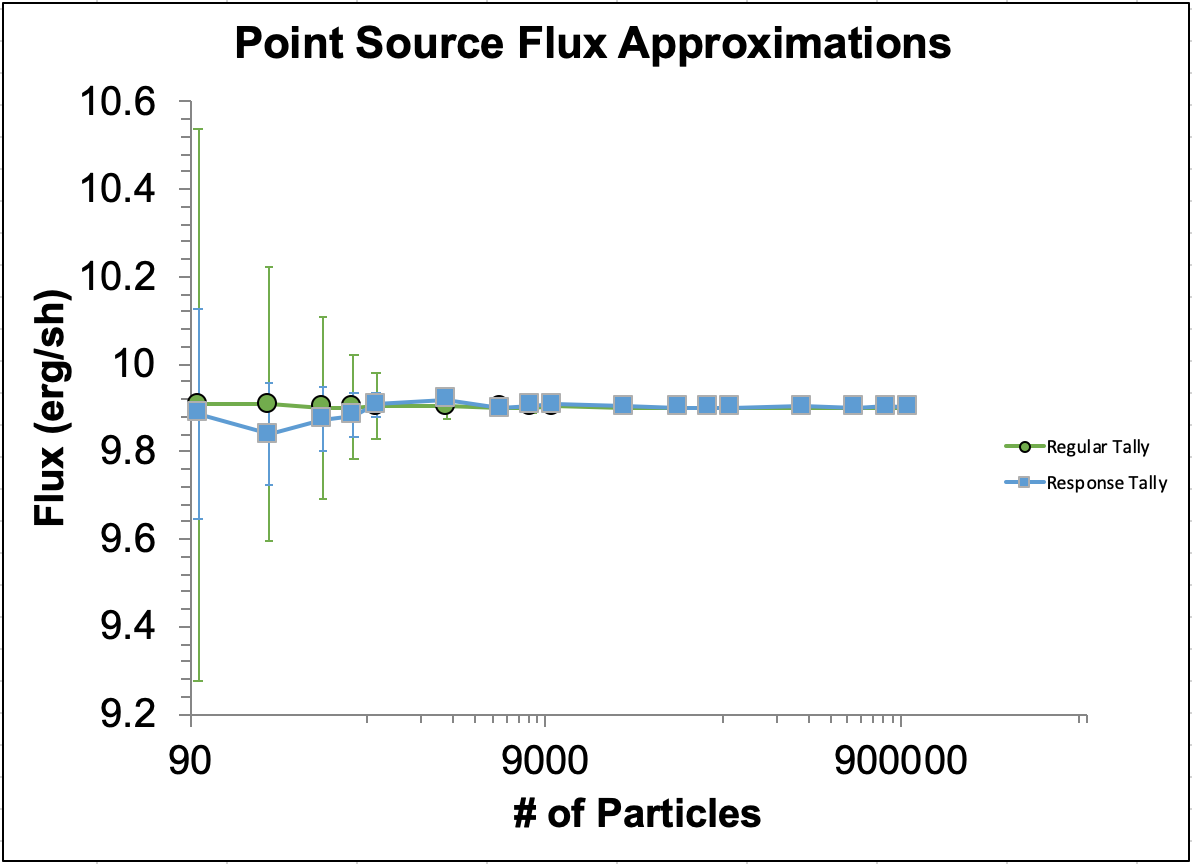
\includegraphics[height=3in]{VarReduction/plots/point_src_errors.png}
	\caption{A graph showing values of the average flux and variance for a point source problem as a function of the number of forward particles simulated. This shows that the response method has far less variance for fewer simulated particles, which implies that it is a more efficient method under these conditions.}
	\label{fig:point_source_errors}
\end{figure}

Results of the average flux and variance testing are shown in Fig. \ref{fig:point_source_errors}. The analytic flux for a point source problem is determined using the following equation:
\begin{equation}
Flux = \frac{Q \exp{-\sigma_{a}}}{A_{tally}}
\end{equation}
where $Q$ is the total source weight, $\sigma_{a}$ is the absorbtion opacity, and $A_{tally}$ is the surface area of the tally. Because the point-source problem is effectively steady-state, average flux and variance were determined from the average over all of the time steps in the simulation. The general trend of this plot demonstrates that the response function produced values largely centered around the analytic flux with significantly lower variance. It should be noted, however, that the second data-point is anomalous: likely resulting from statistics or a minor bug in the code. 

\begin{figure} [h!]
	\centering
	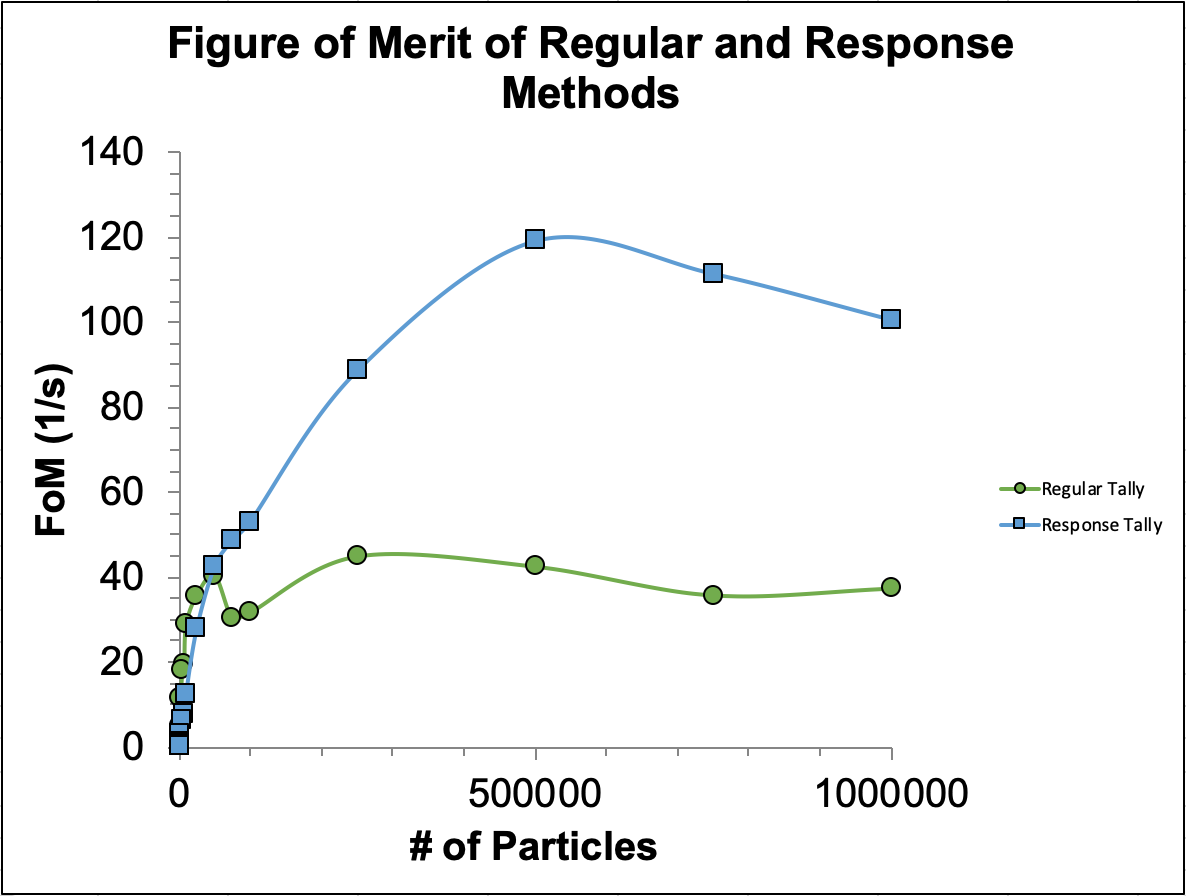
\includegraphics[height=3in]{VarReduction/plots/point_src_fom.png}
	\caption{A graph showing the figure of merits (FoM) of the regular tally method as well as the response function. A higher FoM corresponds to a method that provides less variance in a more efficient period of time. This figure shows that after approx. 50k particles, our method results in a greatly improved FoM compared to a regular tally. This provides a strong basis for the usefulness of our method.}
	\label{fig:point_source_FoM}
\end{figure}

The FoM for the response function is compared to the standard tally method in Fig. \ref{fig:point_source_FoM}. The FoM for the different methods is determined by the following equation outlined in Lewis and Miller 1993 \cite{LM93}:
\begin{equation}
FoM = \frac{1}{\sigma^{2}(x) \cdot t_{run}}
\end{equation}
where $\sigma^{2}(x)$ is the variance of the method and $t_{run}$ is the time to run the simulation. A higher FoM for a method indicates a method that produces an answer more efficiently between variance and run time. As in Fig. \ref{fig:point_source_errors}, this plot also illustrates an improvement of the response function over the standard tally: the FoM of the response function is equivalent to or better than that of the standard tally. At around $\approx 50k$ particles run through the simulation, the FoM of the response function method consistently exceeds that of the standard tally method by more than a factor of $2$.

\begin{figure} [h!]
	\centering
	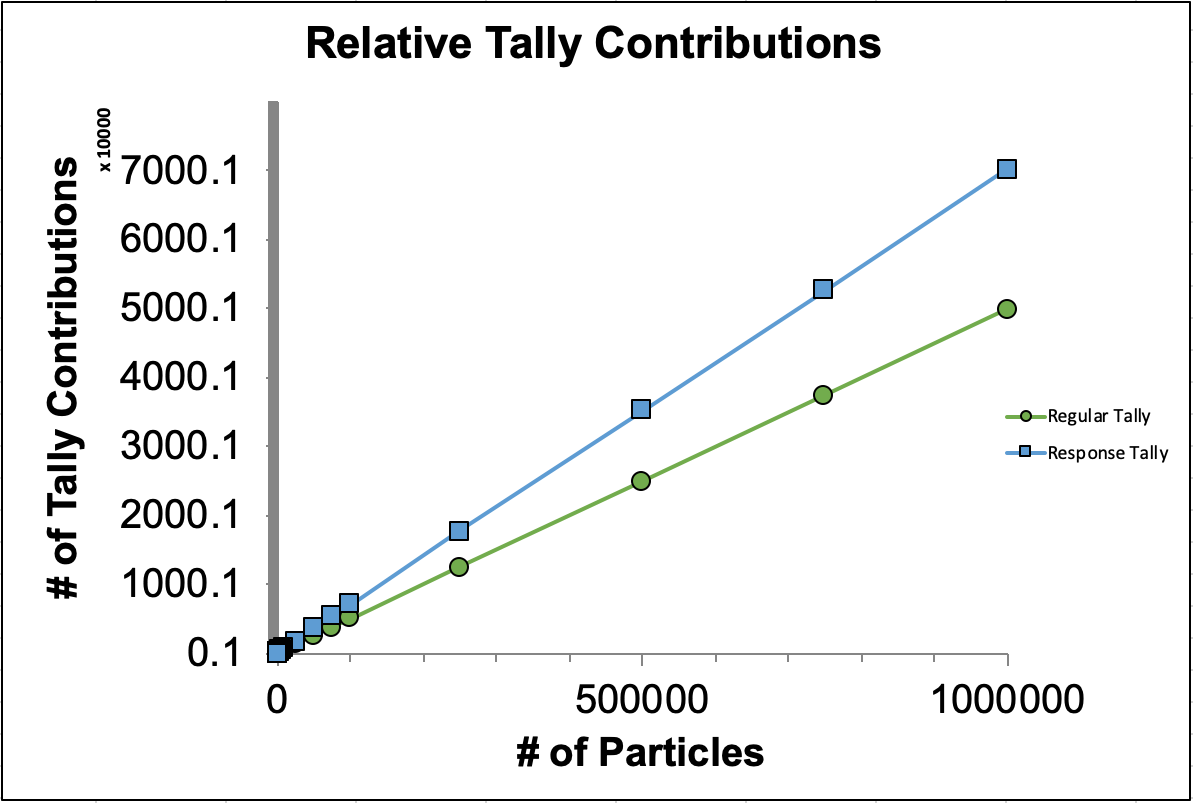
\includegraphics[height=3in]{VarReduction/plots/point_src_contr.png}
	\caption{A graph showing the number of particles (or times in the case of the response function) that contribute to the tally. In general, a method will be expected to have a smaller variance with a greater number of particles that contribute to the tally. }
	\label{fig:point_src_num_contr}
\end{figure}

The results of these two measures provide a strong basis for the validity and usefulness of the response function tally for our simplified point-source problem. Additionally, the integration of the response function theory into the computational method is validated further by Fig. \ref{fig:point_src_num_contr}. Our response function method has a far greater number of contributions ($\approx 40 \%$ greater for the given input variables), matching the intended design for the problem types at hand. Considering the impact of these results gives us a strong foundation to test more complex problems.

\section{Results \& Supernova Applications}
This section presents the results of the response function method applied to a simplified supernova problem. The geometry of the supernova is represented as cubic shells for the ease of the generation of an input file. This problem is further referred to as the 'cubanova' problem. This geometry can be seen on the left-hand side of Fig. \ref{fig:cubanova_op_a}. The innermost shell (yellow) is the supernova eject, the next out is the Ejecta-CSM Shock (red), followed by the CSM (pre-shock) (green) from Table \ref{tab:supernova_params} surrounded by void (blue). The simulation results were compared against standard tally methods as a point of reference. 

\subsection{Cubanova with Spherical Tally}

\begin{figure} [h!]
	\centering
	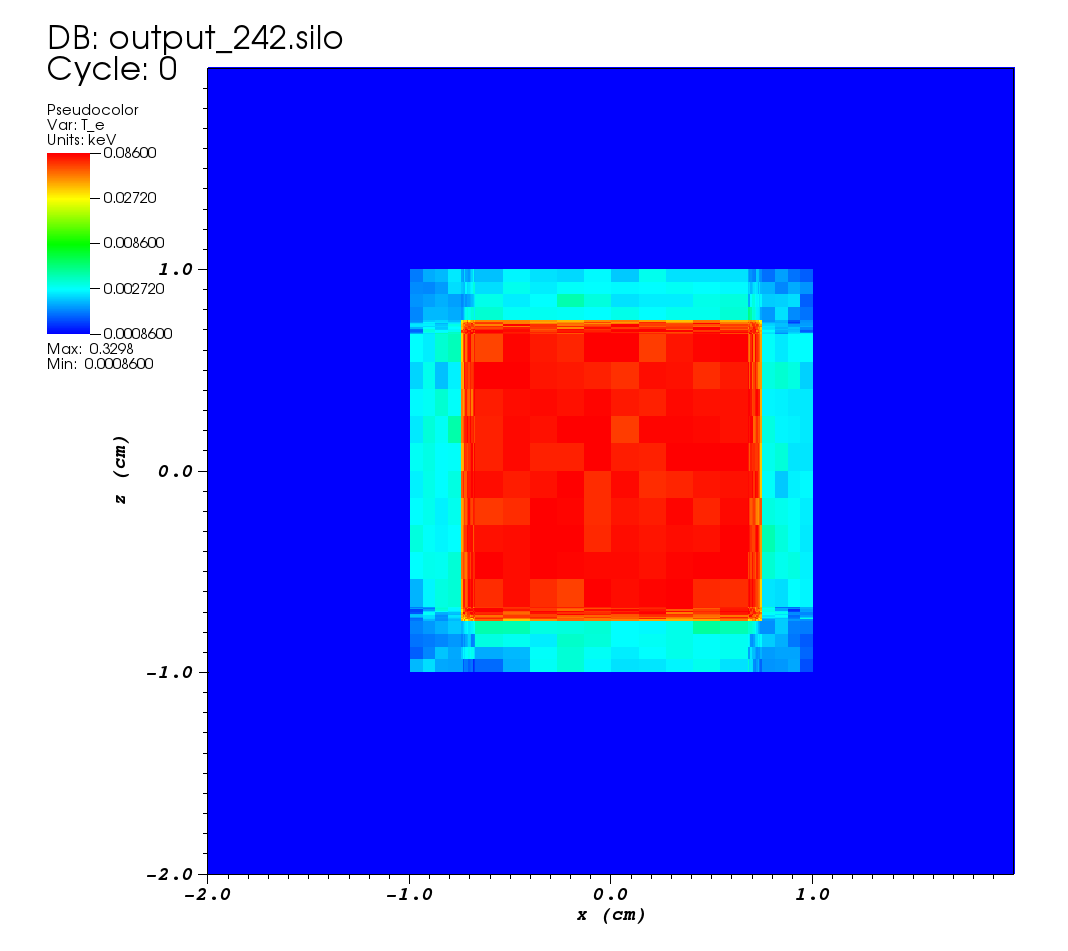
\includegraphics[height=3in]{VarReduction/plots/cubanova_T_e.png}
	\caption{A plot of the electron temperature at the end of the simulations shown in Figs. \ref{fig:cubanova_op_a}, \ref{fig:cubanova_flux_var}, \ref{fig:cubanova_avg_error}. }
	\label{fig:cubanova_T_e}
\end{figure}

\begin{figure} [h!]
	\centering
	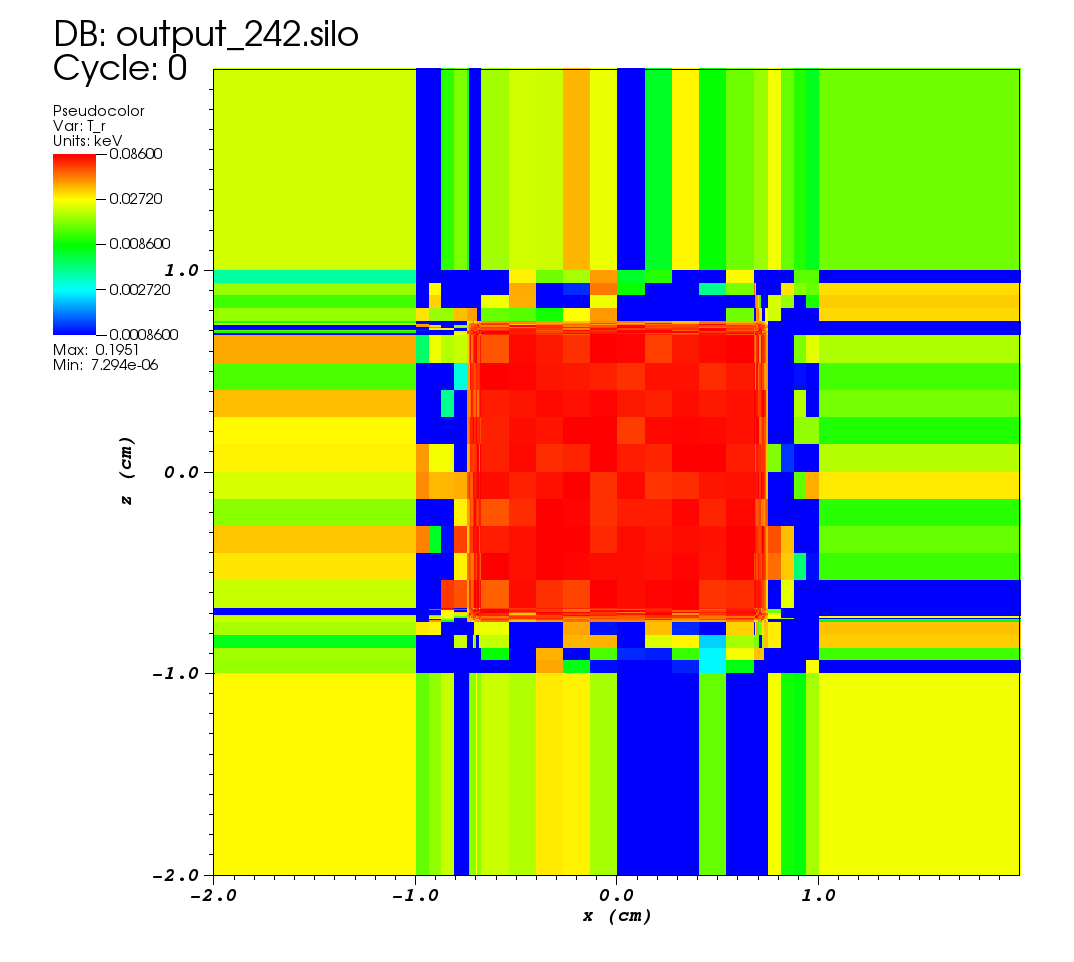
\includegraphics[height=3in]{VarReduction/plots/cubanova_T_r.png}
	\caption{A plot of the radiation temperature for the simulation in Fig. \ref{fig:cubanova_T_e}.}
	\label{fig:cubanova_T_r}
\end{figure}

For these simulations, a spherical tally surface was centered in the problem domain, $(0,0,0)$, with a radius of $2$. The simulations where run at a coarse particle/time-step resolution which results in a significant amount of noise in the radiation and temperature field as shown in Figs. \ref{fig:cubanova_T_e} and \ref{fig:cubanova_T_r}. This plot demonstrates why the response function tally is possibly more efficient than the regular tally for this type of problem: it shows how poorly resolved the radiation solution is outside of the innermost material region.

\begin{figure} [h!]
	\centering
	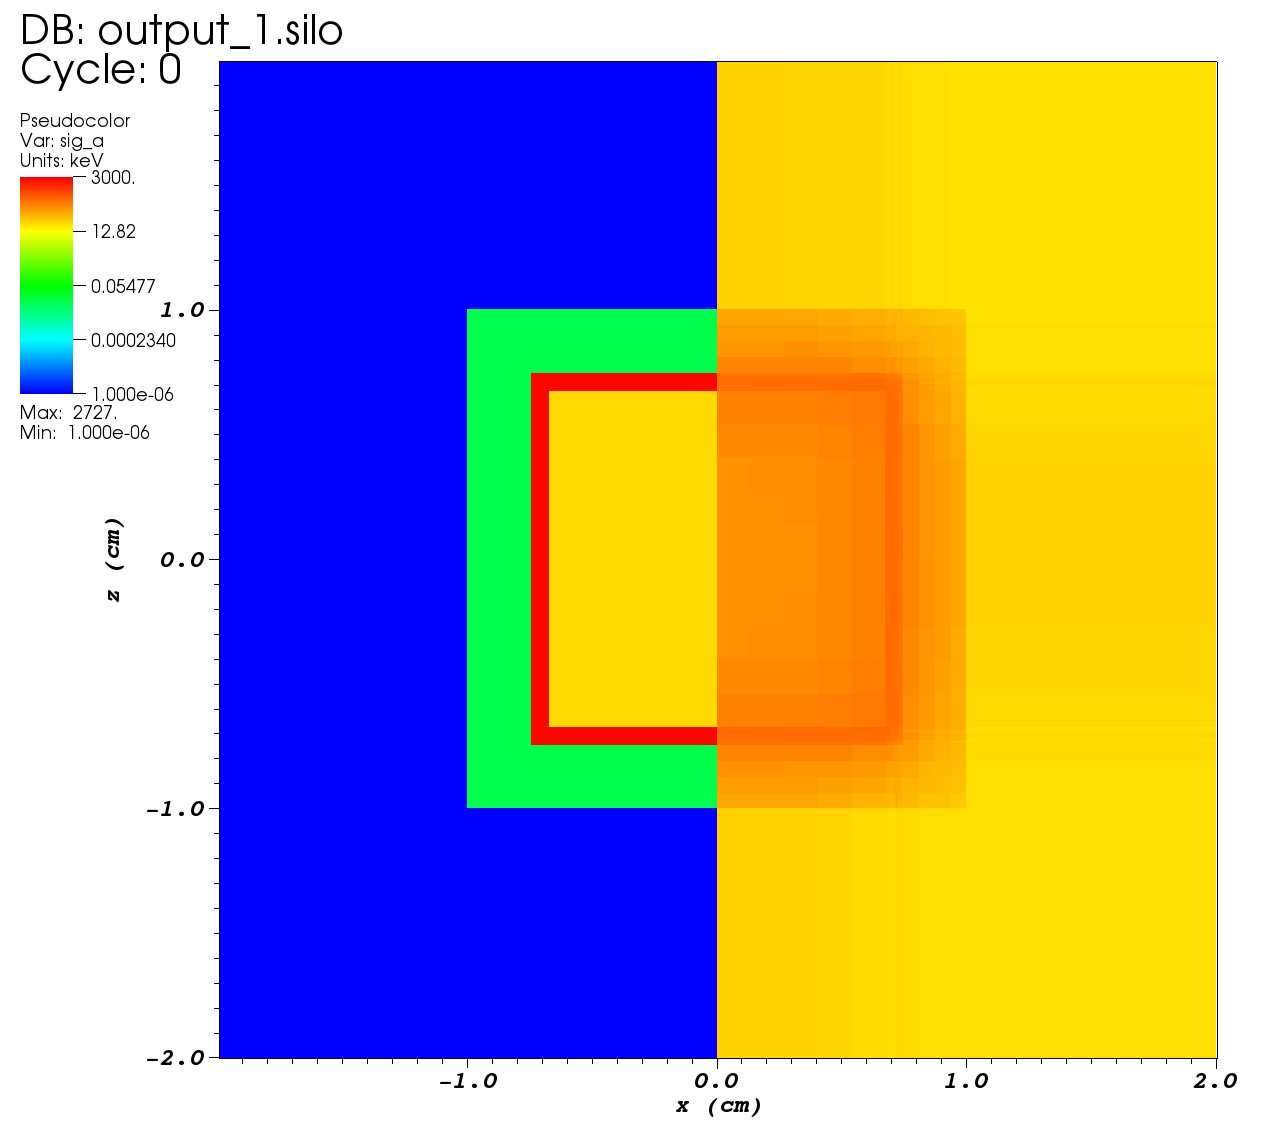
\includegraphics[height=3in]{VarReduction/plots/cubanova_op_a.png}
	\caption{A plot of the geometrically simplified supernova problem showing the true $\sigma_{a}$ value of the problem (left-hand side) as well as the $\sigma_{r}$ values generated by the response function method (right-hand side).}
	\label{fig:cubanova_op_a}
\end{figure}

Figure \ref{fig:cubanova_op_a} shows a comparison between the true $\sigma_{a}$ of the problem at time $t_{0}$ (left-hand side) as well as the generated response values, $\sigma_{r}$, (right-hand side) for each cell. The response value for each cell represents the average opacity between the cell and every possible tally location. 

From a visual standpoint, the response values match expectations. The smearing artifacts along the axis in the response values show a limitation of the direction-independent $\sigma_{r}$ calculation. This in general leads to an under-estimation of the flux in the forward transport problem. This can be slightly aleviated through a directional-dependent $\sigma_{r}$ calculation.

\begin{figure} [h!]
	\centering
	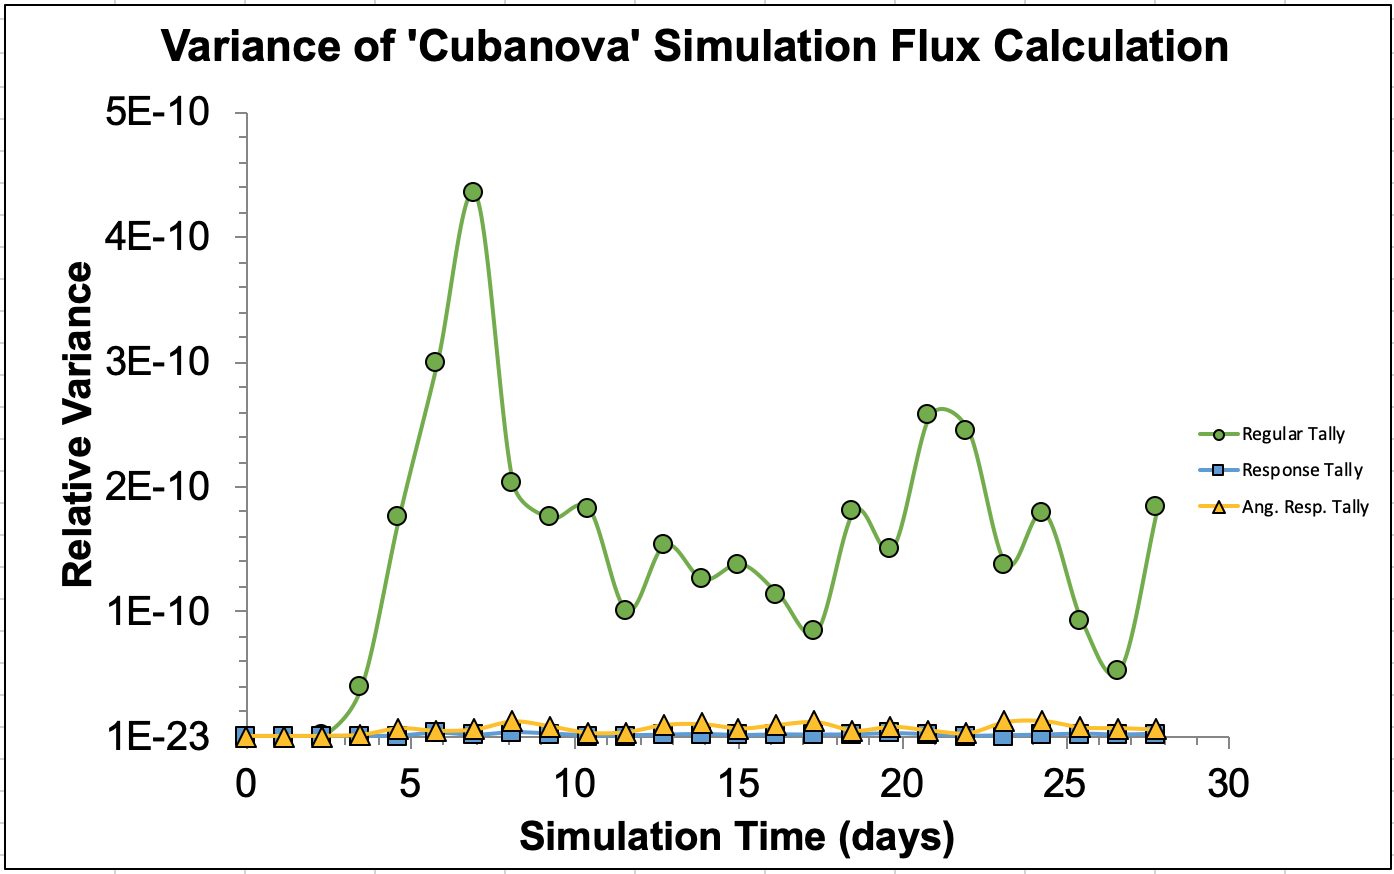
\includegraphics[height=3in]{VarReduction/plots/cubanova_flux_var.png}
	\caption{A graph demonstrating the variance of the regular tally, and response function tally, and an angle dependent response tally for the simplified supernova simulation from Fig. \ref{fig:cubanova_op_a} as a function of the simulation time.}
	\label{fig:cubanova_flux_var}
\end{figure}

Since the flux of the cubanova problem has detailed space- and time-dependence (i.e. there is no analytic flux solution to compare to) the average and variance of each method was calculated for each time step from a number of independent simulations each with a unique random seed. Figure \ref{fig:cubanova_flux_var} shows the results from twenty independent simulations for the standard tally and response tally methods. The general trends indicate that the response function method has a significantly lower variance at any given time step where the flux is statistically meaningful (see Fig. \ref{fig:cubanova_avg_error}). It should also be noted that the variance of the response method is relatively stable compared to that of the regular tally, implying that the response method will be stable and predictable throughout the simulation relative to standard methods. 

\begin{figure} [h!]
	\centering
	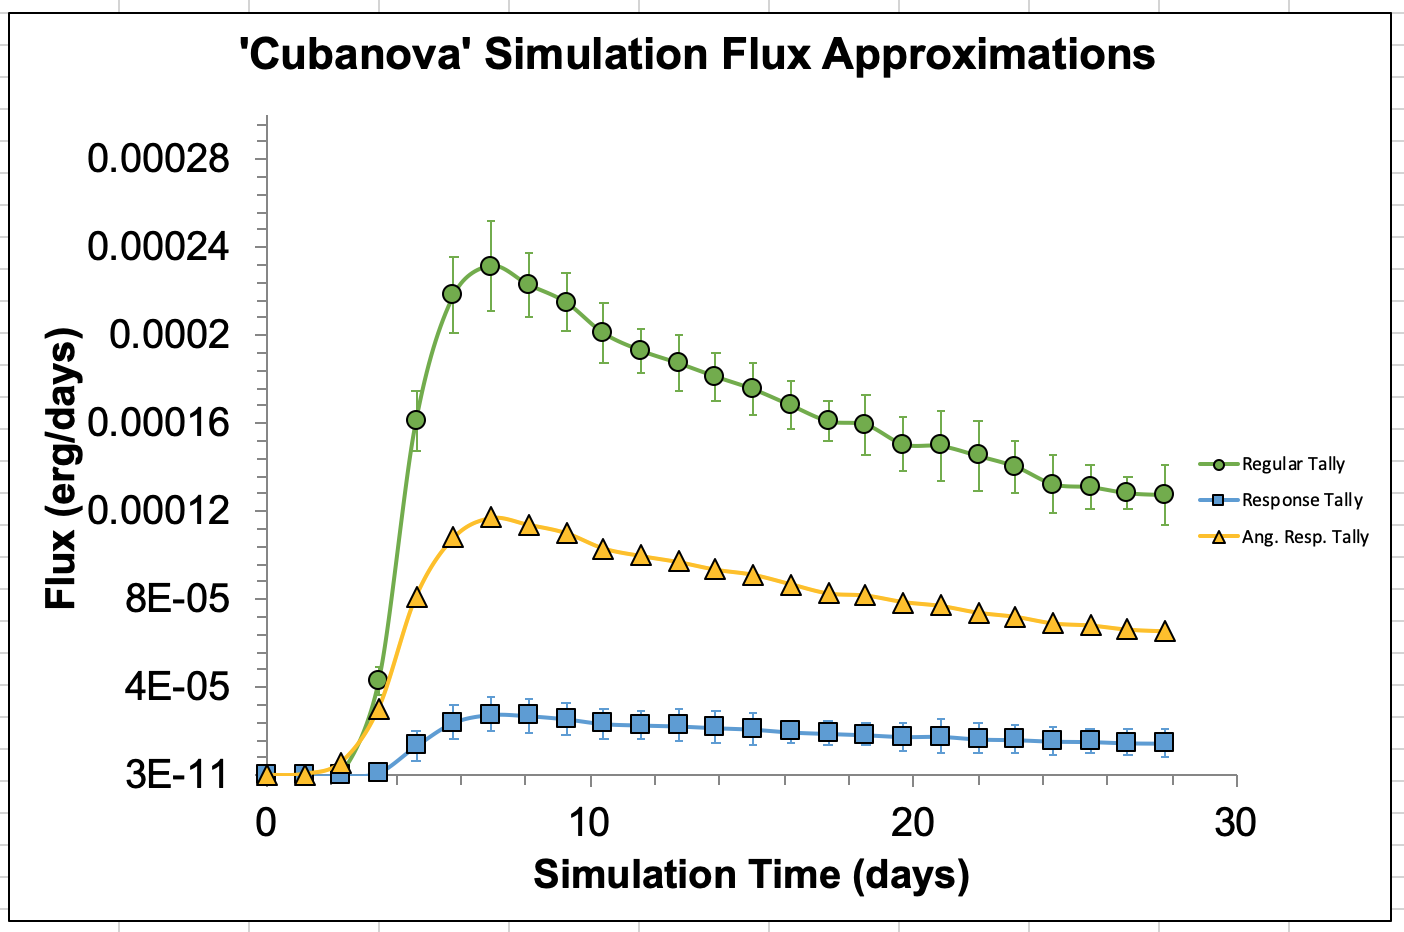
\includegraphics[height=3in]{VarReduction/plots/cubanova_avg_error.png}
	\caption{The relative flux calculations made by the regular tally method and the response function tally method. As in Fig. \ref{fig:point_source_errors}, the response method has a smaller variance, however, it also drastically underestimates the flux. This likely stems from the use of a spherical tally surface instead of a directional tally surface for this particular problem.}
	\label{fig:cubanova_avg_error}
\end{figure}

Figure \ref{fig:cubanova_avg_error} illustrates the average flux and standard deviation from the simulations run in Fig. \ref{fig:cubanova_flux_var}. It is important to note that the response function produces an average flux significantly lower than the standard tally method which is thought to closely approximate the true flux. However, the angle-dependent method does approximate the solution more closely. We believe that this discrepancy is not in the fault of the method, but rather an artifact of the use of a spherical tally on which the response function is generated. Under this, we would expect that a planar tally surface will produce a flux that accurately represents the true value as it has its directionality built-in. Section \ref{Sec: plane_tally} discusses this and results of using a planar tally.

\subsection{Cubanova with Planar Tally} \label{Sec: plane_tally}		
A planar tally is investigated for use in the cubanova simulation as its inherent directionality, in theory, should generate a flux via the response function method that aligns more consistently with the regular tally method. For these simulations, a $YZ$ plane centered at $X = 2$ was used. Additionally, the plane was bounded by the problem region, as otherwise the response function method would contribute to the tally for particles outside the problem domain. 

Due to the directionality of a plane, a slightly modified forward transport method was used: instead of increasing the number of particles in the inverse problem, a photon is simply `marked for response.' Then, a particle contributes to the tally at its birth, every subsequent scattering event, and also if the photon is `marked for response.' After contribution, a particle is no longer `marked for response.' This method was implemented as particles are only traced in one general direction. Small corner cells would then require a significantly longer time to get a contribution, making it computationally inefficient.

\begin{figure} [h!]
	\centering
	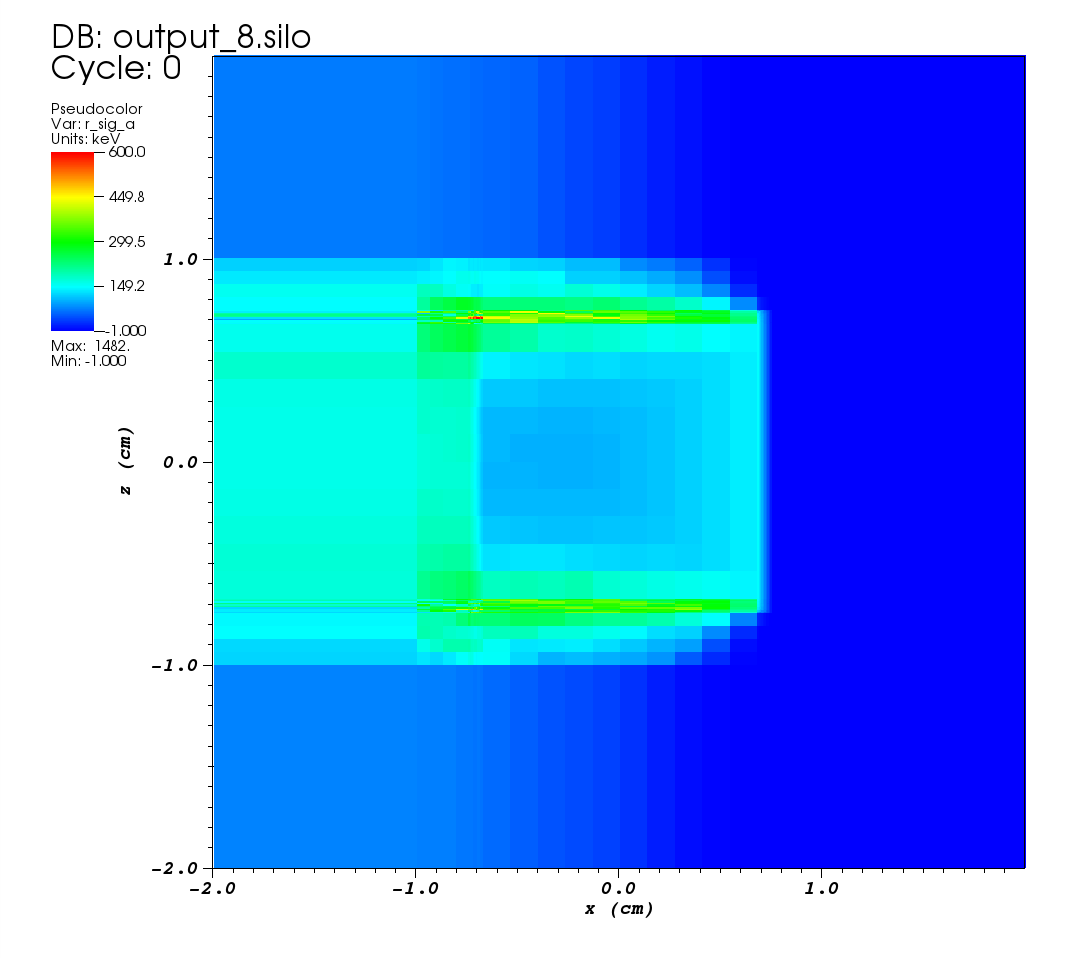
\includegraphics[height=3in]{VarReduction/plots/plane_r_sig_a.png}
	\caption{A plot of the response function values for the cubanova simulation using a $YZ$ planar tally centered at $X=2$. }
	\label{fig:plane_r_sig_a}
\end{figure}

The response function values using the planar tally are shown in Fig. \ref{fig:plane_r_sig_a}. From a visual standpoint, the plot appears as we would expect: smearing in the negative x-direction results from the directionality of the transported particles.

\begin{figure} [h!]
	\centering
	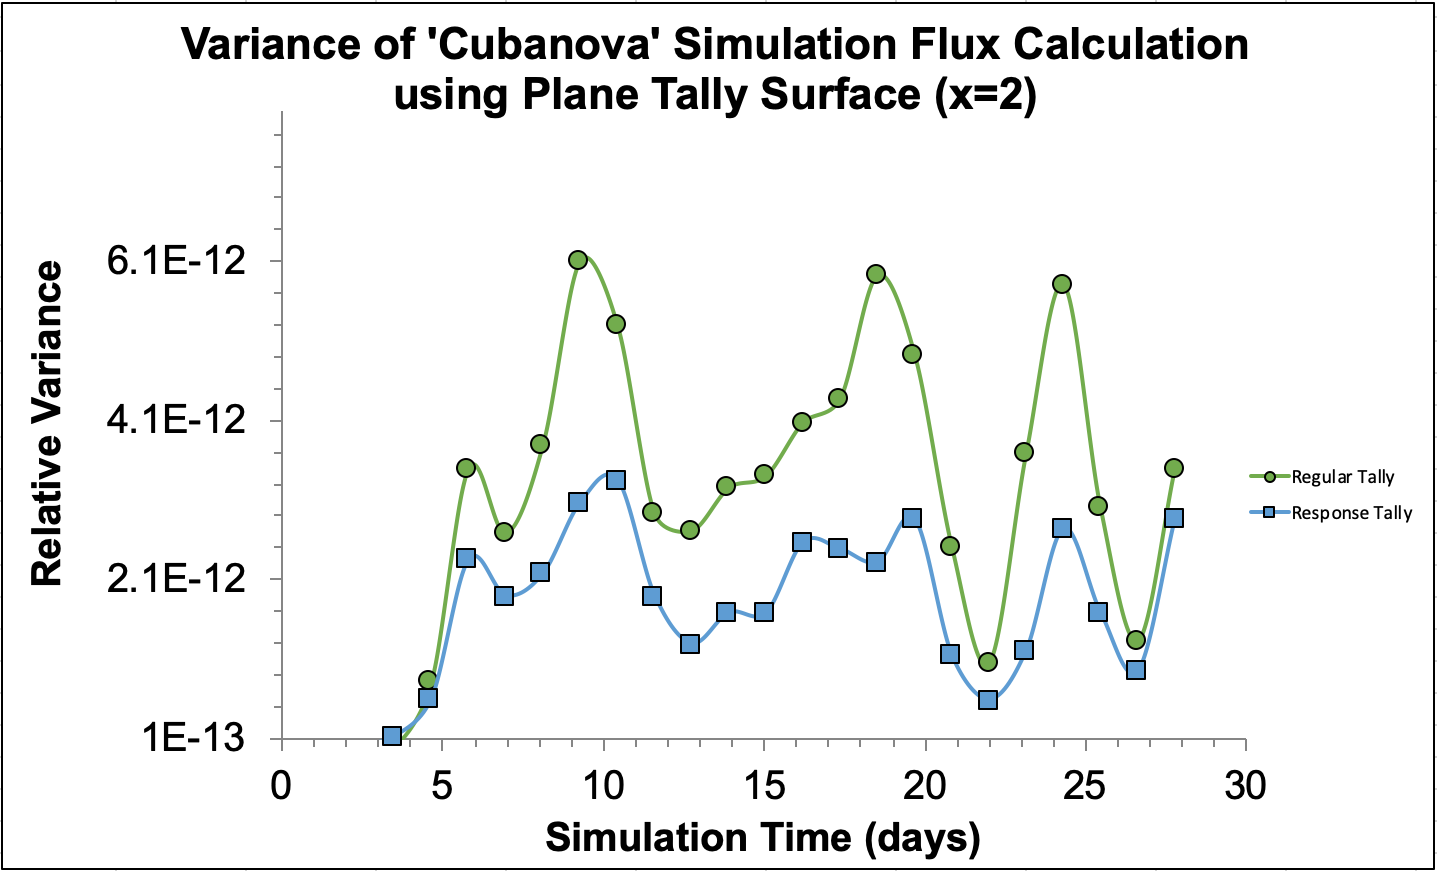
\includegraphics[height=3in]{VarReduction/plots/plane_response_var.png}
	\caption{A graph showing the relative variance of the regular and response function methods using a planar tally along the $YZ$ axis at the edge of the positive x-axis.}
	\label{fig:plane_response_var}
\end{figure}

\begin{figure} [h!]
	\centering
	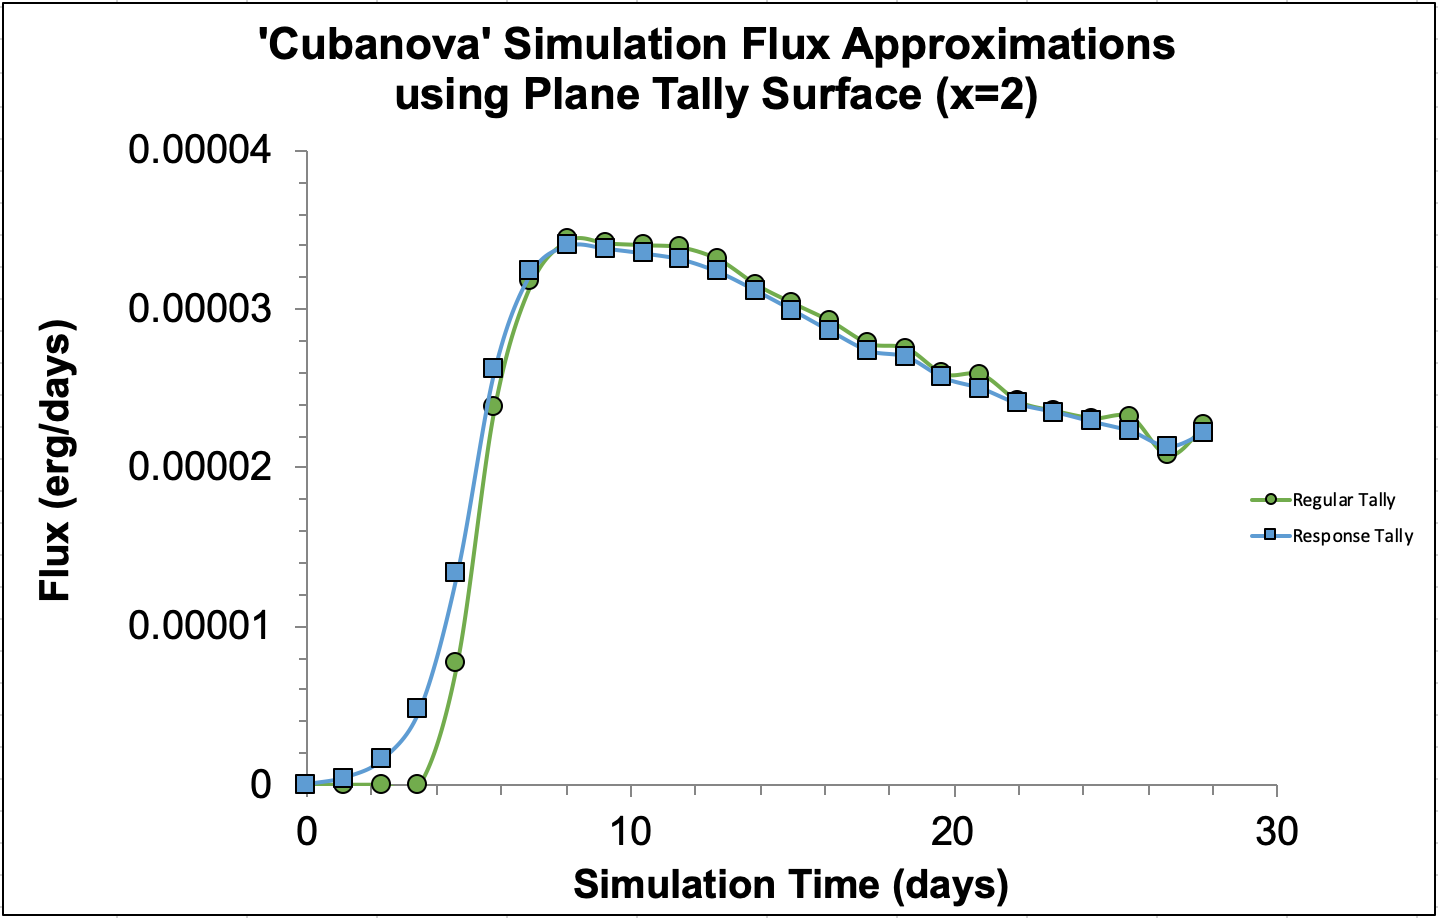
\includegraphics[height=3in]{VarReduction/plots/plane_avg_error.png}
	\caption{A graph showing the calculated flux of the planar response function compared to the standard tally method with the standard deviation of the flux values shown. }
	\label{fig:plane_avg_flux}
\end{figure}

The motivation for using a planar tally is in approximating the problem flux with a lower variance than a regular tally method. Figure \ref{fig:plane_response_var} shows that the variance of the planar tally method is significantly lower than that of the regular tally ($43.9\%$).  Additionally, Fig. \ref{fig:plane_avg_flux} shows the planar tally flux approximation is statistically equivalent ($<1\%$ difference on average) to that of the appoximate analytic solution obtained by the regular tally with a significantly greater number of forward particles. 

It should also be noted that the planar tally recieves approximately four orders of magnitude more particles than the regular tally. For these problems with higher opacities, a more complex problem geometry, and/or limited particle histories, the planar tally becomes of more use. 

\begin{figure} [h!]
	\centering
	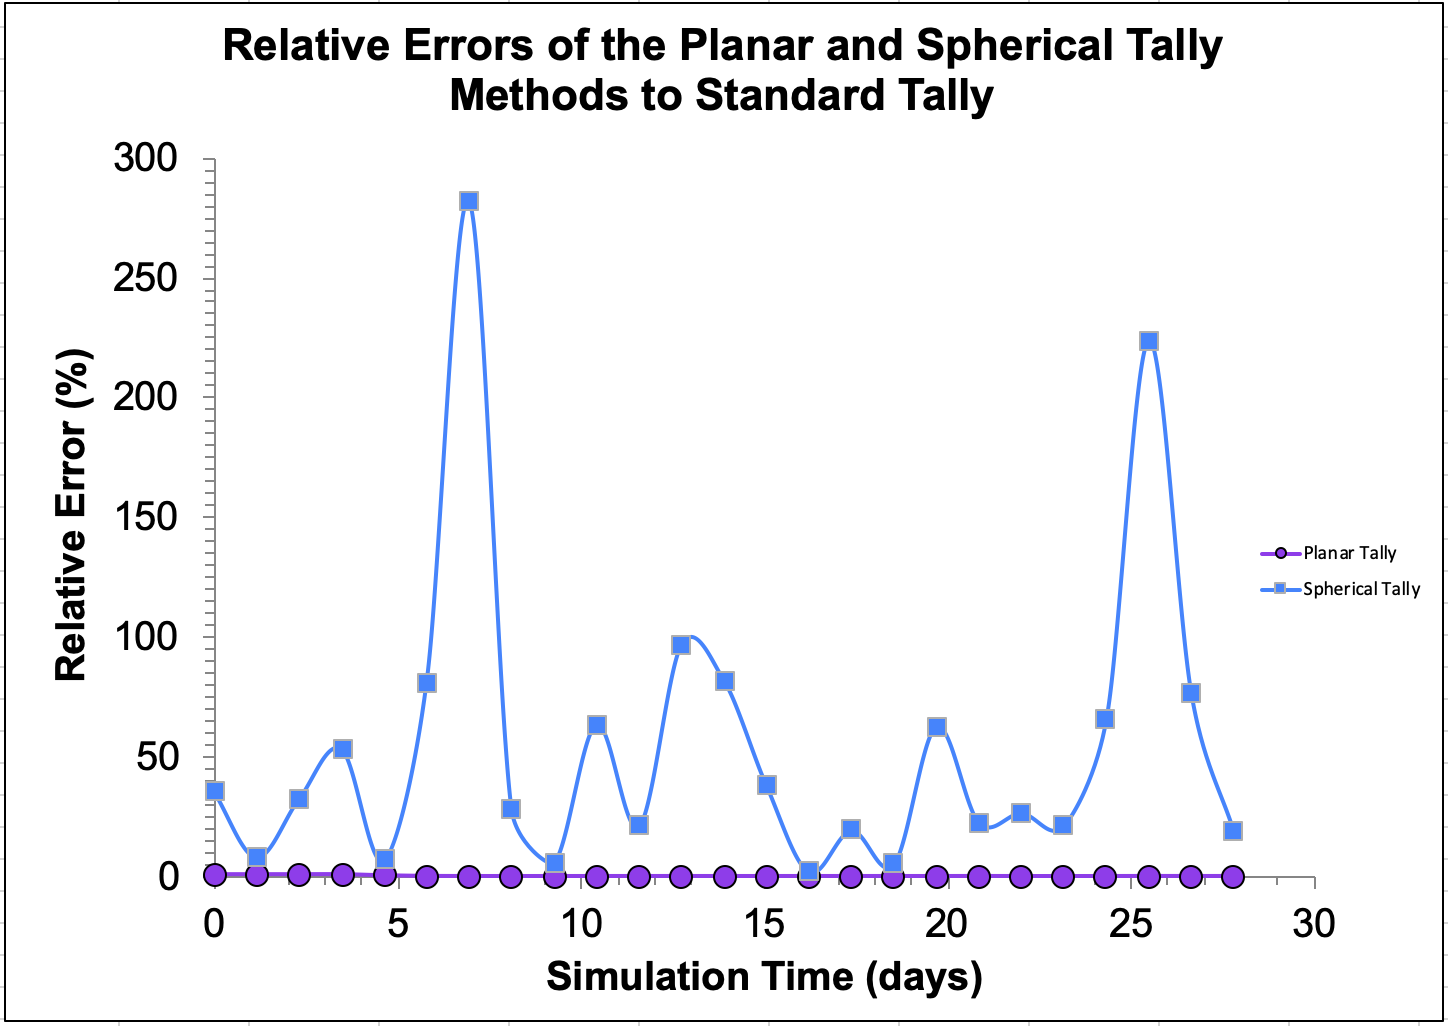
\includegraphics[height=3in]{VarReduction/plots/relative_errors.png}
	\caption{A graph comparing the relative errors of the spherical- and planar-geometry response function tallies for the cubanova simulation. }
	\label{fig:relative_errors}
\end{figure}

These expectations are further validated by Fig. \ref{fig:relative_errors} which shows the relative errors of the average flux calculations for planar and spherical respone function geometries to the regular tally. The general trend clearly indicates that for the cubanova problem, the planar tally consistently produces values closer to the approximate analytic (regular tally method with a significantly greater number of forward particles) than the spherical tally method produces. This also indicates a strong connection between problem and tally geometry with the variance and accuracy of the results obtained. 

\section{Conclusions and Future Work}
Our investigation into the use of a response function-based variance reduction method for use in simulations modeling supernova interactions with its circumstellar medium has shown a notable improvement in variance over standard methods in simple cases. 

The lack of directionality in the response function likely causes the method to under-predict the flux for a spherical tally. The planar tally implementation did demonstrate a closer approximation to the regular tally method, albeit with no improvement of the variance. We do expect that the method will preform better for tally geometries that reflect the geometry of the problem.

Future work will include looking at improving the directionality of the response function for different problem and tally geometries. It would be very useful to perform a response mesh resolution study in angle and energy to determine when the response tally result ``converges'' to the regular tally. Optimization of the response function generation method could also be performed. Additionally, running our response function with a more realistic supernova-CSM simulation to determine if our method converges accordingly is of interest as well.

\Bios{Scott E. Campbell}{is an rising junior at Gonzaga University in Spokane, Washington, with a double major in Physics and Math-Computer Science.}%
{}{}

%-----------------------------------------------------------
% Each team's report has its own bibliography.  You must have these
% two lines to add your team's bibliography.
\bibliographystyle {plainnat}
\bibliography{VarReduction/references}

